\chapter{Preprocessing}\label{chapter:preprocessing}
This chapter describes, how the data has been collected and what steps have been done to transform the data, so that it is suitable for training models.

\section{Data collection}
\subsection{Environment}
During creating benchmarking data, it is necessary to create the same conditions, at each run of the program. Preferably, the data generation occurs on dedicated machines, where little to no other background processes can impact the performance of the benchmarking program. This approach has been taken in this thesis, where the data generation, occurs only at times, where no other user is using the same machine concurrently. This was ensured, by registering who uses the machine at a table on a shared tabular scheduling sheet. The table \ref{tab:system_info} describes the hardware and software characteristics of the server machine running the data generation program. 

\begin{table}[h]
\centering
\begin{tabular}{|l|l|}
\hline
\textbf{Characteristic} & \textbf{Value} \\ \hline
CPU Product & AMD Ryzen 9 7950X 16-Core Processor \\ \hline
CPU Vendor & Advanced Micro Devices [AMD] \\ \hline
CPU Cores & 16 \\ \hline
CPU MHz & 3360.195 \\ \hline
Total Memory & 64 GB \\ \hline
OS Description & Ubuntu 23.10 \\ \hline
Architecture & x86\_64 \\ \hline
Linux Kernel version & 6.5.0-15-generic \\ \hline
\end{tabular}
\caption{Benchmarking Server System Information}
\label{tab:system_info}
\end{table}

\subsection{Binary programs}
After making sure that the data can be collected consistently, the subsequent phase involves thinking about how the data is to be collected. For the purpose of this thesis, program binaries have been provided, which execute the B+ tree configuration behavior as defined by Müller et al. \parencite{mueller2024}. Each binary file executes a b-tree configuration using the inputs and 
produce output a multi-line string in the comma-separated format containing input configuration together with the measured outputs. More details on the operations being benchmarked are provided in section \ref{subsec:ycsb}.
The input and the output values are further outlined in feature tables, table \ref{tab:input_features_example} and table \ref{tab:output_features_example}. In the feature tables, for numerical and boolean features, if only one value is provided as an example, this feature is not varied in further context. 
\\\\
Each run of a single binary gives an output in three lines. The first line describes the header of the comma-separated values. The second and third contain the inputs and output in the comma-separated format of the initialization of the operation and the actual operation, respectively.
\\\\
When calling a binary program, some of the input parameters are embedded in the binary itself, in which case changing it requires a call to a different binary. This is the case for the inner and leaf node page size and the configuration (eg. hints, head). The rest of the parameters are passed to the binary program by setting environment variables beforehand. 
\begin{table}[H]
\centering
\resizebox{\textwidth}{!}{
\begin{tabular}{|l|l|l|}
\hline
\textbf{Feature} & \textbf{Description} & \textbf{Example Value(s)} \\ \hline
bin\_name & Name of the binary & \texttt{bins/-DPS\_I=4096 -DPS\_L=4096/hints-n3-ycsb} \\ \hline
config\_name & set of optimizations &  hash, hints, baseline, prefix, dense3\\ \hline
const\_basicHintCount & Basic hint count & 16 , 0 \\ \hline
const\_enableBasicHead & Enable basic head optimization& 1 \\ \hline
const\_enableDense & Enable dense optimization& 0 , 1 \\ \hline
const\_enableDense2 & Enable dense 2 optimization& 0 \\ \hline
const\_enableDensifySplit & Enable densify split & 0 , 1 \\ \hline
const\_enableHash & Enable hash optimization & 0 , 1 \\ \hline
const\_enableHashAdapt & Enable adapation optimization & 0 \\ \hline
const\_enableHeadNode & Enable head node optimization& 0 \\ \hline
const\_enablePrefix & Enable prefix truncation optimization & 1 \\ \hline
const\_hashSimdWidth & SIMD operation width & 32 \\ \hline
const\_hashSortUseStdMerge & Hash sort use standard merge & 1 \\ \hline
const\_hashUseCrc32 & Hash use CRC32 & 0 \\ \hline
const\_hashUseSimd & Hash use SIMD & 1 \\ \hline
const\_headNode4HintCount & Head node 4 hint count & 16 \\ \hline
const\_headNode8HintCount & Head node 8 hint count & 16 \\ \hline
const\_pageSizeInner & Inner node page size & 2048, 4096, 8192 \\ \hline
const\_pageSizeLeaf & Leaf node page size & 2048, 4096, 8192 \\ \hline
data\_name & Name of the data & data/urls, int \\ \hline
data\_size & Size of the data, key count &  5181932, 2813666\\ \hline
data\_sorted & Data sorted status & 0 \\ \hline
density & Density & 0.5, 0.75, 1 \\ \hline
op & Operation & ycsb\_c, ycsb\_c\_init, ycsb\_e, ycsb\_e\_init \\ \hline
payload\_size & Size of values & 8, 256 \\ \hline
rand\_seed & Random seed & 1703378455, 1703378098 \\ \hline
run\_id & Run ID & fc16dbaa-104b-4777-8087-bbe953b81b16 \\ \hline
ycsb\_range\_len & YCSB range length & 100 \\ \hline
ycsb\_zipf & YCSB zipf & 0.9, 0.651367 \\ \hline
\end{tabular}
}
\caption{Input Features with Example Values}
\label{tab:input_features_example}
\end{table}



\begin{table}[H]
\centering
\resizebox{\textwidth}{!}{
\begin{tabular}{|l|l|l|}
\hline
\textbf{Feature} & \textbf{Description} & \textbf{Example Value(s)} \\ \hline
time & Time in seconds &  1.0512e-06, 3.126e-07 \\ \hline
nodeCount\_X & Node count of type X & 19755, 20879 \\ \hline
counted\_final\_key\_count & Final key count & 5798920, 3175985 \\ \hline
cycle & Average number of CPU cycles pro operation & 2197.381, 1087.615 \\ \hline
instr & Average CPU instructions pro operation & 1927.571 1151.517 \\ \hline
X\_miss & Average misses pro operation in cache type X  & 43.867, 9.918  \\ \hline
task & Kernel execution time & 392.291, 194.439 \\ \hline
scale & Scale &  5798920, 10000000 \\ \hline
IPC & Instructions Per Cycle & 0.877, 1.059 \\ \hline
CPU & CPU usage & 1, 0.993, 0.99 \\ \hline
GHz & CPU frequency & 5.601, 5.594 \\ \hline
\end{tabular}
}
\caption{Output Features with Example Values}
\label{tab:output_features_example}
\end{table}


\subsection{Data generation program}

Collecting the data is done through a Python script that runs in a loop, that terminates after a configured timeout. Inside the loop, the input parameters are generated either with a constant, or depending on the use case randomly from a given set, or a random value in a range. The outputs are collected and appended to three different files: the error logging file, the output file and the logging of the script file. Each file serves a purpose. The error logging file is useful to identify issues with the binaries that are called. The output file contains the data that is later analyzed. The logging of the script file is useful to identify issues of the Python script itself. \\ \\
Two versions of this script exist that set the generation of the input parameters for the specific use case. For general model building more values are generated at random, whereas for the analysis of the page size, the values are more fixed to be able to be able to better make use of discrete data mining algorithms.\\ \\
The Python script is called in a Poetry \parencite{poetry:online} environment and to make the script run in the background the \textit{nohup} \parencite{nohup1Li95:online} command is utilized.\\ \\
Once the script is finished running, the output files are checked to verify a successful run. Since the following steps do not require a consistent environment, the output files are copied to a local device, where the output is further processed, analyzed and other experiments are run.

\subsubsection{ML model program}
For the use case of training the \ac{ML} models, the input parameters are set to the following values:

\begin{itemize}
    \item \textbf{ycsb\_zipf}: Random value between 0 and 1.5 
    \item \textbf{op}: The operations \textit{c} with \textit{c\_init} are chosen twice as much as \textit{e} with \textit{e\_init} 

    \item \textbf{data\_name}: Set statically to \textit{data/urls}

    \item \textbf{const\_pageSizeLeaf}: Randomly varied in powers of two between 2048 and 16384 
    \item \textbf{const\_pageSizeInner}: Randomly varied in powers of two between 2048 and 16384 
    \item \textbf{payload\_size}: Set statically to 8
    \item \textbf{density}: Generated with \texttt{ 1 / 2 ** random()}
    \item \textbf{config\_name}: Randomly chosen between \textit{dense3}, \textit{hints} and \textit{hash}
    \item \textbf{data\_size}: Generated by \texttt{ floor((10 ** (random() * 0.5 + 8.25))/ 70.280)}. \texttt{70.280} corresponds to an estimated average size of a key.  
\end{itemize}

\subsubsection{Pattern recognition program}
For the use case of using data mining techniques, and reasons stated in section \ref{patternreg}, the input parameters are varied the following way:  
\begin{itemize}
    \item \textbf{ycsb\_zipf}: Set statically to 1 
    \item \textbf{op}: The operations \textit{c} with \textit{c\_init} are chosen twice as much as  \textit{e} with \textit{e\_init} 
    \item \textbf{data\_name}: Set statically to \textit{data/urls}
    \item \textbf{const\_pageSizeLeaf}: Randomly varied in powers of two between 2048 and 8192 
    \item \textbf{const\_pageSizeInner}: Randomly varied in powers of two between 2048 and 8192 
    \item \textbf{payload\_size}: Randomly varied in powers of two between 4 and 256
    \item \textbf{density}: Set statically to 1
    \item \textbf{config\_name}: statically set to \textit{hints}
    \item \textbf{data\_size}: Randomly generated in 1 million steps between 1 and 6 million. 
\end{itemize}


\section{Aggregate data}

After the files are collected in a subfolder, all following steps are done in Jupyter Notebooks \parencite{jupyter:online}, to enable quick step-by-step running of the programs. There are two steps that are done: \\ \\
In the first step, the multiple output files, originating from multiple data generation script runs, are merged into one file. This step is done by traversing the subfolders and finding files matching the naming convention defined for the specific types of the generation script. The files are then merged by appending the lines of each file to an array and then writing the array into a new file.\\\\
The second step, takes the new merged file and removes the excessive header lines that are caused by each run of a binary creating its own header line. Additionally, in this step excessive spaces are removed, to make the output format in accordance with a comma-separated values (.csv) file type. This way libraries like \textit{pandas} \parencite{pandasdo55:online} and consequently \textit{scikit-learn} \parencite{scikitle99:online}, and \textit{mlxtend} \parencite{mlxtend35:online} can read and process the given data. 

\section{Cleanup data}

After aggregating the data into one file, the data needs to be cleaned up, to be more suitable for \ac{ML} models. For the use case of this thesis, multiple aspects need to be considered to make sure that the ML models, do not learn from data, that is invalid, wrongly interpreted or unavailable for the considerations of the use-case. These considerations are implemented using the \textit{pandas} library \parencite{pandasdo55:online}. After reading the data into a DataFrame, the following steps are done: \\
 
\begin{itemize}
    \item \textbf{Remove failed runs}: Binary program executions that have run into an error during benchmarking occasionally produced outputs, that are to be considered outliers and irrelevant for model training. These executions are easily identified, because of the feature \textit{time} being equal to 0. Therefore, these records are filtered out of the DataFrame. 
    \item \textbf{Rescale time into time per op}: One important aspect to consider is the feature \textit{time}. This feature is the total time that the program took to perform the benchmark. This, however, is highly correlated to the number of records being inserted or read. The total time, is not representative of the time, which this thesis aims to optimize. Instead, this needs to be transformed into the time per operation. This is done by dividing the feature \textit{time} by the feature \textit{scale}. For simplicity, the result overwrites the values for the feature \textit{time}. 
    \item \textbf{Reduce complexity of input}: When training some \ac{ML} models, it is best practice to reduce the number of dimensions to reduce the number of records needed to get a performant model. There are ways to do this is with algorithms that reduce the dimensionality by projecting the higher dimensionality space into lower dimensions, trying to preserve the main information. One example, according to Bishop \parencite{bishopML}, is PCA, but another, simpler way is to perform feature selection, as proposed by Murphy \parencite{murphy2012machine}. This refers to dropping features that based on domain knowledge are known to not contribute to the end result. In this case, for the input features, it is only the feature \textit{bin\_name}.  
    \item \textbf{Drop output features}: Another necessary step in \ac{ML} is to ensure that the models are not getting information, that in the use-case, it would not have without knowing the result. In the case of this thesis, it is important to not feed models information, that is generated during the output of the binary program executions. This means that all output features, except the target feature \textit{time}, are dropped out of the DataFrame. The importance of this step is further outlined in section \ref{correlationchapter} on correlation.
\end{itemize}

\section{Encoding categorical data}
Since some features are not numeric and are categorical, in order to be able to train \ac{ML} models on the preprocessed data, they need to be converted into numerical values. The approach chosen in this thesis is \textbf{one-hot encoding}, as described by Murphy \parencite{murphy2012machine}. As a consequence, the amount of features is increased, however since only a few features are affected, and the features themselves, only contain a few categories, the number of features increased from 28 to 33.

\section{Separate YCSB operations}\label{subsec:ycsb}

The binary programs execute \ac{ycsb} benchmarking programs as introduced by Cooper et al. \parencite{ycsb}. \ac{ycsb} can be configured for different workloads, which the figure \ref{fig:ycsb} describes together with an example, where such a distribution of operations can occur. In this thesis, the feature \textit{op} describes which workload is being measured. The main focus for this thesis is the workload C and secondarily the workload E is considered as well. This corresponds to the values \textit{ycsb\_c} and \textit{ycsb\_e} in feature \textit{op}. The initial population of the B+ tree is also benchmarked and represented by values \textit{ycsb\_c\_init} and \textit{ycsb\_e\_init} respectively in feature \textit{op}.
\begin{figure}[h]
  \centering
  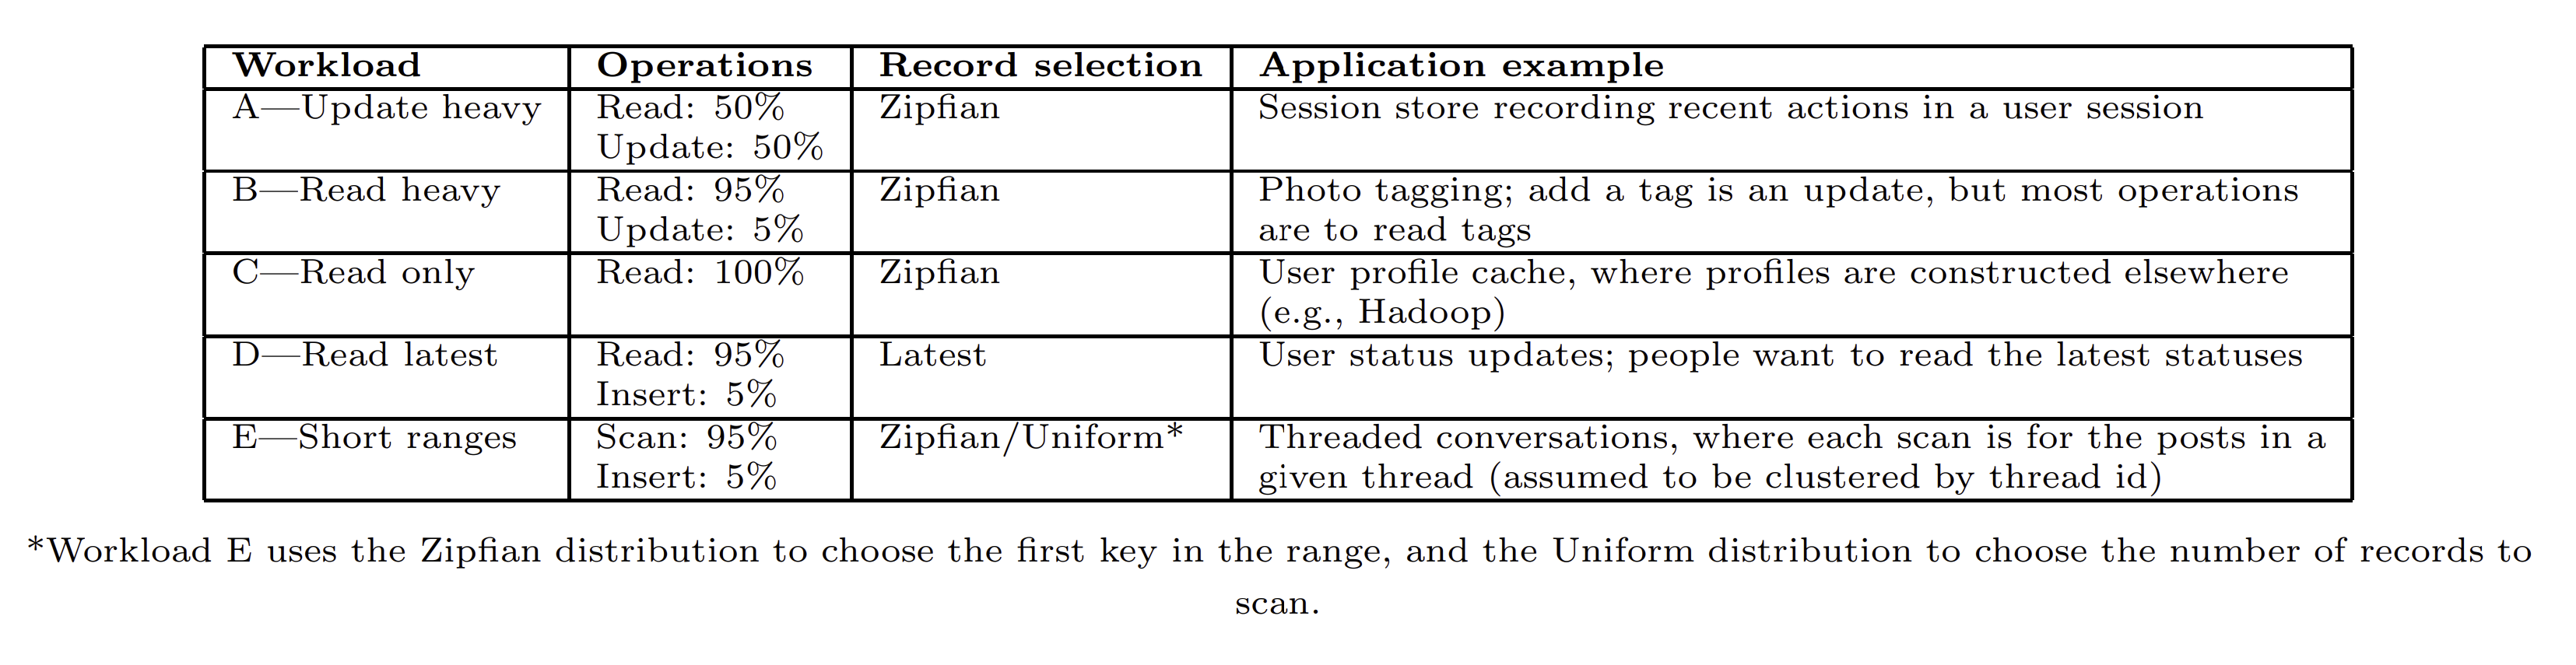
\includegraphics[width=0.8\textwidth]{images/ycsb.png}
  \caption{Definition of types of \ac{ycsb} workloads \parencite{ycsb}}
  \label{fig:ycsb}
\end{figure} 
\\\\
One early observation during the initial analysis was that the operation being benchmarked has a big influence on the measured \textit{time}. The idea of the thesis, however, is to find interpretable insights into which configurations influence the \textit{time} and how. Since the \textit{op} has a significant impact, and different configurations might benefit some operations more than others, the dataset is split into parts according to the feature \textit{op} and all the models are trained based on the respective parts. The box plot in figure \ref{fig:optime} represents the measured time of records for each operation type. The visible shift for each operation type, further supports the reason for splitting the data set, by highlighting the impact of single feature \textit{op} on the feature \textit{time}.

\begin{figure}[h]
  \centering
  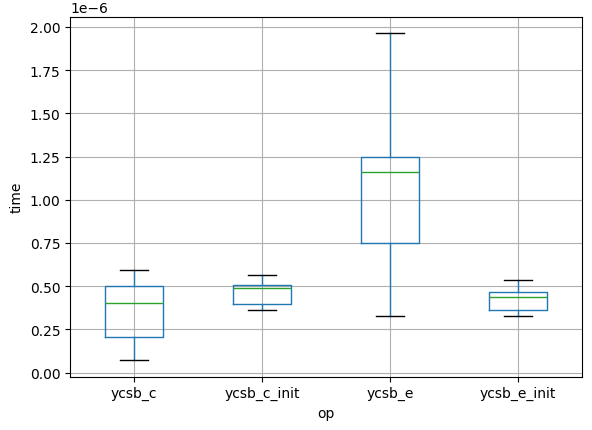
\includegraphics[width=0.5\textwidth]{images/boxplot_op.png}
  \caption{Box plot of time grouped by feature \textit{op}}
  \label{fig:optime}
\end{figure} 